\chapter{Plotting}
\index{plotting}
\label{c:plotting}

\tao has a graphical display window within which such things as lattice functions, machine layout,
beam positions, etc., can be plotted. An example is shown in \fig{f:plot.typ} where there are plots
of the beta function and orbit along with a ``lattice layout which shows the longitudinal positions
of lattice elements. 

\tao uses a software toolkit called \vn{quick_plot} for plotting. Detailed information on this is in
section~\sref{s:quick.plot}.

\clearpage

\begin{figure}[tb]
  \centering
  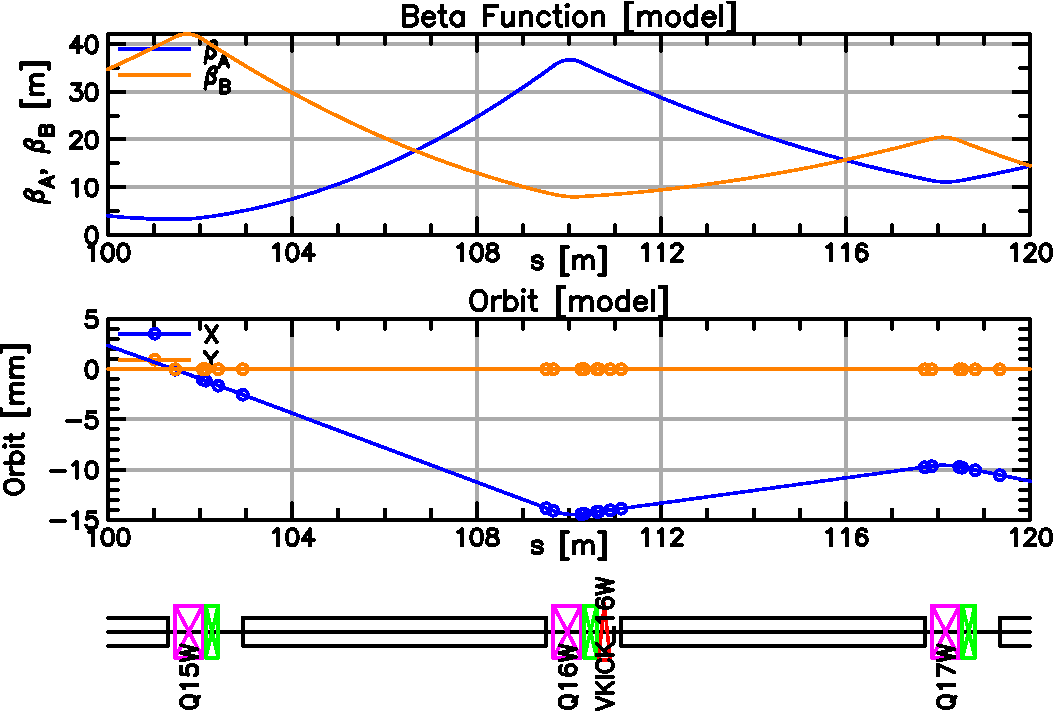
\includegraphics[width=5.0in]{plot-typical.pdf}
  \caption[An example of a plot display.]
{In this example there are three plot: A plot displaying the beta funciton, a plot displaying the orbit, and
a plot displaying the ``lattice layout'' which shows the longitudinal positions of lattice elements.}
  \label{f:plot.typ}
\end{figure}

\begin{figure}[bt]
  \centering
  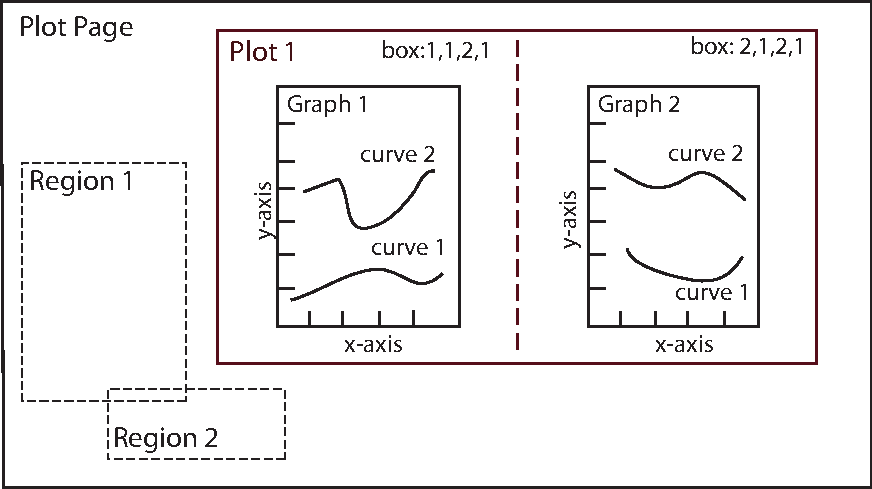
\includegraphics[width=5.0in]{plot.pdf}
  \caption[Plotting nomenclature.]
{The \vn{plot page}, which is the whole display window, has a number of rectangular \vn{regions} in
which a \vn{plot} can be placed. A plot has a collection of graphs and a graph has a collection of curves. A plot
template becomes visible when it is associated with some region on the page using the \vn{place}
command. Note that on the actual page the plot/region border is not visible.}
  \label{f:plot}
\end{figure}

\begin{description}
\index{plot page|hyperbf}
\item[Plot Page] \Newline
The \vn{plot page}, sometimes called the \vn{plot window}, refers to the window where graphics are
displayed or the corresponding printed graphics page. A \vn{plot page} is shown schematically in
\fig{f:plot}. Parameters associated with the \vn{plot page} are discussed in \sref{s:plot.page}.
These parameters may be set in an initialization file or may be set on the \tao command line using
the \vn{set plot_page} (\sref{s:set.plot.page}) command. The \vn{show plot -plot_page} command may
be used to view the paramters.
%
\index{region}
\item[Region] \Newline
The \vn{plot page} is divided up into a number of rectangles called \vn{regions}. \vn{Regions}
define the locations where \vn{plots} may be placed. This is shown schematically in \fig{f:plot}
which shows two regions. Each region has a name and information on where the region is on the plot
page. Regions may be defined by the user. In addition, for convienience, \tao will define a number
of regions. With one exception, all of the \tao defined regions will begin with the letter
'r'. Regions may overlap. How to define regions is explained in \sref{s:plot.page}. The \vn{show
plot} command will show the region list.
%
\index{plot|hyperbf}
\item[Plot] \Newline
A \vn{plot} is essentially a collection of \vn{graphs}. This is shown
schematically in \fig{f:plot} which shows a plot with two graph and \fig{f:plot.typ} shows a plot
page with three plots. 

Plots are divided into two groups. A \vn{template} plot defines how a \vn{displayed} plot is to be
constructed. That is, a \vn{template} plot defines what the associated \vn{graphs} are, defines
graph placement, etc. When a \vn{template} plot is \vn{placed} in a \vn{region}, using the
\vn{place} command, the information of the \vn{template} is copied in order to construct a
\vn{displayed} plot. A given \vn{template} plot may be placed in multiple \vn{regions} to give
multiple \vn{displayed} plots and then, using \vn{set} commands, the data displayed in each of these
plots may be manipulated separately. For example, one displayed orbit plot could show the orbit of
the \vn{model} lattice while another orbit plot could show the orbit difference between the
\vn{model} and \vn{design} lattices. When a \vn{plot} is displayed in a given \vn{region},
everything drawn is scalled to the region size.

Use the \vn{show plot} to see what displayed plots are associated with what regions. Use the
\vn{show plot -templates} command to see a list of \vn{template} plots. \tao defines a number of
default \vn{template} plots. Section~\sref{s:templates} discussses how to define custom template
plots in an initialization file. Use the \vn{set plot} command to modify either \vn{template} or
\vn{displayed} plots.

All plots have a name. A \vn{displayed} plot will inherit the same name of the \vn{template} plot it
came from. A \vn{displayed} plot can be be referred to by using the associated \vn{region} name. If there
is an ambeguity, 

%
\item[Box] \Newline
To determine where a \vn{graph} is drawn with respect to the boundaries of its associated \vn{plot},
each \vn{graph} is associated with a given \vn{box}. A \vn{box} is a rectangular sub-region of the
\vn{plot}. Boxes are defined by dividing the \vn{plot} into a rectangular grid and then choosing one
of the grid rectagles to be the \vn{box} associated with the \vn{graph}. The is illustrated in
\fig{f:plot} where \vn{Graph 1} of \vn{Plot 1} is associated with the box with label
``\vn{1,1,2,1}''.  The last two digits of a \vn{box} label (\vn{2,1} here) specify the number of
rectangles grid has horizontally and vertically (2 horizontally, 1 vertically here). The first two
digits (\vn{1,1} here) specify the particular rectangle associated with the \vn{box} with \vn{1,1}
designating the lower left. Different \vn{graphs} do not have to use the same grid to select a box
from.
%
\index{graph|hyperbf}
\item[Graph] \Newline
A \vn{graph} is a diagram of some sort.  Most \vn{graph}s consists of horizontal and vertical axes
along with one or more \vn{curve}s. \vn{Floor_plan} (\sref{s:floor.plan}) and \vn{lat_layout}
\vn{graphs}, on the other hand, shows the placement in space of the lattice elements and do not have
any associated \vn{curves}. A given \vn{plot} will contain a number of \vn{graphs}. For example, in
\fig{s:plot} the plot labeled \vn{plot 1} is shown to have two graphs.

How many \vn{graphs} is assocaited with a \vn{plot} is a matter of convienience and different
\vn{graphs} of a \vn{plot} may display different types of information. For example, it would be
possible to have a single \vn{plot} contain three \vn{graphs} and look like what is shown in
\fig{f:plot.typ}.

How to define \vn{graphs} when defining \vn{template} plots is given in \sref{s:template}. The
\vn{show graph} command can be used to show graph parameters. The \vn{set graph} command can
be used to modify \vn{graph} parameters.
%
\index{curve|hyperbf}
\item[Curve] \Newline
A \vn{curve} is a data set to be displayed within a \vn{graph}. For example, a \vn{curve} may be the
beta function of the \vn{model} lattice. \vn{Curves} have an associated set of points at which a
symbol can be drawn and/or a curved line that can be drawn. For example, in \fig{f:plot.typ} only
the line is drawn with the two curves of the beta plot while both symbols and line are drawn for the
two curves of the orbit plot (here the data points are the orbit at the edges of the lattice elements).

How to define \vn{curves} when defining \vn{template} plots is given in \sref{s:template}. The
\vn{show curve} command can be used to show curve parameters. The \vn{set curve} command can
be used to modify \vn{curve} parameters.
%
\end{description}


Figures~\ref{f:plot.page1} and \ref{f:plot.page2} show examples of a plot
\vn{page}. Figure~\ref{f:plot.page1} was generated by defining two regions called \vn{top}
and \vn{bottom} in the plot initialization file. The \vn{top} region was defined to cover
the upper half of the \vn{page} and the \vn{bottom} region was defined to cover the bottom
half. \vn{Template plots} were defined to plot phase and orbit data from a defined set of
detector elements in the lattice. Each \vn{template plot} defined two graphs which in both
cases where assigned the names \vn{x} and \vn{y}. The orbit \vn{template plot} was placed
in the \vn{top} region and the phase \vn{template plot} was placed in the \vn{bottom}
region. The horizontal axis numbering is by detector \vn{index}.  Displayed plots are
referred to by the \vn{region} name (\vn{top} and \vn{bottom} in this case). Individual
graphs and curves are referred to using the nomenclature \vn{region.graph.curve}. Thus, in
this example, the horizontal orbit graph would be referred to as \vn{top.x}.  Using the
\vn{set plot}, \vn{set graph}, or \vn{set curve} commands (\sref{s:set}) one can then
specify what \vn{components} are plotted. ``\vn{component}'' refers to \vn{measured},
\vn{reference}, \vn{model}, \vn{base}, and/or \vn{design} data (\sref{s:plot.data}).
Notice that the same \vn{template plot} can be assigned to different \vn{regions} and the
plots in different \vn{regions} can have different scales for their axes or different
\vn{components}. In the example in Figure~\ref{f:plot.page1}, the \vn{component} for the
\vn{top} plot is \vn{model} and for the \vn{bottom} plot it is \vn{model - design}.

A displayed plot may be referred to by its name or by the name of the region it is placed in. For
example, the orbit plot in Figure~\ref{f:plot.page1} may be referred to using the region name
(\vn{top}) or the plot name (\vn{orbit}). A template plot may be referred to by its name. Commands,
like the \vn{set plot} command (\sref{s:set.plot}), will first match a plot name to displayed plots
and, if found, will not try to match the name to any template plots. If it is desired to set the
attributes of a template plot while there is a displayed plot of the same name, the prefix
``\vn{T::}'' can be used to direct \tao to ignore displayed plots and only match to template plots.
For example:
\begin{example}
  set plot T::orbit component = design
\end{example}

A template may be placed in multiple regions.  For example, you may wish to plot the \vn{model} data
for the orbit in one region and the \vn{design} data for the orbit in another region. In this case
the command \vn{scale orbit} would scale the plots in both regions while to scale the plot in only
one of the regions you would need to use the region name.

A graph of a plot is specified using the format \vn{plot_name.graph_name} where
\vn{plot_name} is a template or region name and \vn{graph_name} is the name of the
graph. For example, if the horizontal orbit graph of the \vn{orbit} plot is named \vn{x}
then it would be referred to as \vn{orbit.x} or \vn{top.x}. If a plot has only one graph,
the graph may be specified by just using the plot name.

A curve within a graph is specified using the format
\vn{plot_name.graph_name.curve_name}. If a graph has only one curve, the curve may be
specified using only the graph name \vn{plot_name.graph_name}. Additionally, if the there
is only one curve in a plot, the curve can be specified by just using the \vn{plot_name}.

The \vn{use}, \vn{veto}, \vn{restore}, and \vn{clip} commands are used to control what
data is used in fitting the model to the data in the optimization process (see
Chapter~\ref{c:opti}). The general rule is that these commands only affect measured and
reference data. If plotting \vn{model}, \vn{design} and/or \vn{base} data then the data
will be displayed irregardless. If plotting \vn{meas} and/or \vn{ref} data then the data
displayed will vary with these commands.  \vn{meas} or \vn{ref} data vetoed for display is
also vetoed for fitting.  However, measured data that is off the vertical or horizontal
scale may still be used by the optimizer unless vetoed with the \vn{veto} or \vn{clip}
command.  If there are data points off the vertical scale then ``**Limited**'' will appear
in the upper right-hand corner of the graph. If plotting measured data then these points
off scale will still be used by the optimizer.

The \vn{x_axis} and \vn{x_scale} commands are used to set the axis type and scale for each
graph. The axis type can be either \vn{index}, \vn{ele_index} or \vn{s} which corresponds
to the data index number, element index number and longitudinal position in the lattice
(from element 0) respectively.

Figure~\ref{f:plot.page2} shows another example of a plot \vn{page}.  In this case the
\vn{page} was generated by again defining two vertically stacked regions but in this case
the regions have different heights.  A \vn{template plot} with a single graph was placed
in the bottom most \vn{region}.  This \vn{graph} contains a \vn{key_table}.  A
\vn{key_table} is used in conjunction with \vn{single mode} and is explained in
Chapter~\sref{c:single}. A \vn{template plot} containing five \vn{graphs} was placed in
the uppermost region. The uppermost \vn{graph} of this \vn{template plot} contains a
\vn{lat_layout} which shows the placement of lattice elements.  What elements are
displayed in a \vn{lat_layout} and what shapes they are represented by is specified in the
initialization file. The horizontal scale is longitudinal position (\vn{s}).  The
remaining four graphs show dispersion and beta data from two different universes
representing the low energy and high energy transport in an energy recovery linac. The
individual data points here (hard to see in this example) have been slaved to the
\vn{lat_layout} and represent the beta and dispersion at the edges of the displayed
elements in the \vn{lat_layout}.

%-----------------------------------------------------------------
\section{Quick_Plot Plotting}
\label{s:quick.plot}

\vn{Quick_Plot} is an interface library developed for \bmad for graphics plotting. 

QuickPlot uses
the following concepts:
\begin{example}
  PAGE  -- The entire drawing surface.
  PLOT  -- A rectangle defined with respect to the PAGE within which graphs are placed.
  BOX   -- For each GRAPH associated with a given PLOT, the GRAPH defines a two-dimensional array of BOXes that
            partition the PLOT. The GRAPH is positioned with respect to a given BOX in this array. 
            Each GRAPH can define a different two-dimensional array of B0Xes.
  GRAPH -- The actual plotting rectangle where curves are drawn within the bounds of the axes.
\end{example}

%-----------------------------------------------------------------
\subsection{Length and Position Units}
\label{s:qp.units}

For text that has an associated \vn{justify} parameter, the \vn{justify} parameter is a two
character string.  The first character gives the horizontal justification:
\begin{example}
   "L" -- Left justify
   "C" -- Center justify
   "R" -- Right justify
\end{example}
The second character gives the vertical justification
\begin{example}
   "B" -- Bottom justify
   "C" -- Center justify
   "T" -- Top justify
\end{example}

For text that has an associated \vn{units} parameter, the \vn{units} parameter is a character string
which is divided up into three parts. The syntax of the \vn{units} parameter is:
\begin{example}
   "unit_type/ref_object/corner"
\end{example}
Where \vn{unit_type} is the type of units:
\begin{example}
   "%"       - Percent.
   "DATA"    - Data units.
   "MM"      - millimeters.
   "INCH"    - Inches.
   "POINTS"  - Printers points (72 points = 1 inch, 1 pt ~ 1 pixel).
\end{example}
\vn{ref_object} is a reference object (optional except if \vn{unit_type} = "\%").
\begin{example}
   "PAGE"  -- Relative to the plot display window.
   "BOX"   -- Relative to the box the graph is associated with.
   "GRAPH" -- Relative to the graph rectangle.
\end{example}
And \vn{corner} is the origin location (optional):
\begin{example}
   "LB" -- Left Bottom.
   "LT" -- Left Top.
   "RB" -- Right Bottom.
   "RT" -- Right Top.
\end{example}

%-----------------------------------------------------------------
\subsection{qp\_point\_struct}
\label{s:qp.point}

\vn{QuickPlot} defines a number of structures to parameterize such things like line and symbol
properties.

The \vn{qp_point_struct} defines where a point is:
\begin{example}
  type qp_point_struct:
    x     = <real>     ! Horzontal offset of point from fiducial point
    y     = <real>     ! Vertical offset of point from fiducial point
    units = "<units>"  ! Fiducial point position and units of x \& y.
\end{example}
Example:
\begin{example}
  graph%curve_legend_origin = 5.0, -2.0, "POINTS/GRAPH/LT"
\end{example}
In this example the fiducial point the left-top point on the graph rectangle. The
\vn{curve_legend_origin} is positioned 5.0 points horizontally to the left and 2.0 points vertically
downward from this fiducial point.

%-----------------------------------------------------------------
\subsection{qp\_axis\_struct}
\label{s:qp.axis}

The \vn{qp_axis_struct} structure defines the properties of a graph axis
\begin{example}
  type qp_axis_struct::
    label             = "<string>" ! Axis label string.
    min               = <real>     ! Min is the left or bottom axis number.
    max               = <real>     ! Max is the right or top axis number.
    number_offset     = <real>     ! Offset from axis line in inches.
    label_offset      = <real>     ! Offset from numbers in inches.
    major_tick_len    = <real>     ! Major tick length in inches.
    minor_tick_len    = <real>     ! Minor tick length in inches.
    label_color       = <string>   ! Color of the label string
    major_div         = <integer>  ! Number of major divisions
    major_div_nominal = <integer>  ! Major divisions nominal value.
    minor_div         = <integer>  ! Minor divisions. 0 = Tao will choose.
    minor_div_max     = <integer>  ! Max minor div number if Tao chooses.
    places            = <integer>  ! Number of digits to print
    type              = <string>   ! Axis type: "LINEAR" or "LOG".
    bounds            = <string>   ! Axis bounds: "GENERAL", "ZERO_AT_END", etc.
    tick_side         = <integer>  ! 1 = draw to the inside, 0 = both, -1 = outside.
    number_side       = <integer>  ! 1 = draw to the inside, -1 = outside.
    draw_label        = <logical>  ! Draw the label string
    draw_numbers      = <logical>  ! Draw the numbers.
\end{example}

The \vn{%bounds} parameter sets how the axes min and max values are calculated when plots are initially
instantiated and when \vn{scale}, \vn{x_scale}, and \vn{xy_scale} commands are used. Possible settings
are:
\begin{example}
  "ZERO_AT_END"      ! Min or max value is set to zero.
  "ZERO_SYMMETRIC"   ! Min and max chosen so that max = -min.
  "GENERAL"          ! No restrictions (default).
  "EXACT"            ! The User min/max is used.
\end{example}
If input min and max values are specified by the User, \tao will take the specified values as the starting
point to find ``nice'' min and max values to use. For example, with the command
\begin{example}
  scale all 0 19
\end{example}
and with \vn{bounds} set to \vn{"GENERAL"}, the min and max values will be set to 0 and 20. The exception is when
\vn{bounds} is set to \vn{"EXACT"}. In this case the User supplied min and max values will be used as is.

Examples:
\begin{example}
Tao> set graph r13 y%bounds = "zero_at_end"
Tao> scale r13 200 280   ! Graph bounds set to [0, 300]

Tao> set graph r13 y%bounds = "zero_symmetric"
Tao> scale r13 200 280   ! Graph bounds set to [-300, 300]

Tao> set graph r13 y%bounds = "general"
Tao> scale r13 20 190    ! Graph bounds set to [0, 200]

Tao> set graph r13 y2%bounds = "exact"
Tao> scale r13 -y2 20 190    ! Y2 graph bounds set to [20, 190]
\end{example}

%-----------------------------------------------------------------
\subsection{qp\_point\_struct}
\label{s:qp.point}

\begin{table}
\begin{tabular}{ll} \toprule
{\B}u       & Start a superscript or end a subscript \\[0.3ex]
{\B}d       & Start a subscript or end a superscript.
              {\B}u and {\B}d must always be used in pairs \\[0.3ex]
{\B}b       & Backspace (i.e., do not advance text pointer  
               after plotting the previous character) \\[0.3ex]
{\B}fn      & Switch to Normal font (1)       \\[0.3ex]
{\B}fr      & Switch to Roman font (2)        \\[0.3ex]
{\B}fi      & Switch to Italic font (3)       \\[0.3ex]
{\B}fs      & Switch to Script font (4)       \\[0.3ex]
{\B}{\B}    & Backslash character (\B)        \\[0.3ex]
{\B}x       & Multiplication sign ($\times$)  \\[0.3ex]
{\B}.       & Centered dot ($\cdot$)          \\[0.3ex]
{\B}A       & Angstrom symbol (\AA)         \\[0.3ex]
{\B}gx      & Greek letter corresponding to roman letter x. See Table~\ref{t:greek}. \\[0.3ex]
{\B}mN {\B}mNN & Graph marker number \vn{N} or \vn{NN} (1-31) \\[1ex]
{\B}(NNNN)  & 
\parbox{5.2in} {Character number NNNN (1 to 4 decimal digits) from the Hershey character set which
includes a number of special characters including mathematical, musical, astronomical, and
cartographical symbols.} \\ \bottomrule
\end{tabular}
\caption{Escape Sequences for Labels.}
\label{t:plot.escape}
\end{table}

The \vn{major_div} parameter is not settable directly. Rather, \vn{major_div_nominal} may be set by
the user and then \tao will calculate the value of \vn{major_div} such that the value of
\vn{major_div} is ``close'' to the value of \vn{major_div_nominal} with the constraint that the value
of \vn{major_div} ``nicely'' divides the range from given by the values for \vn{min} and \vn{max}.

The \vn{places} parameter set the number of places to display a number. \tao will automatically
calculate this number and it is not user settable.

The \vn{label} parameter may include Greek letters, subscripts, superscripts, and special characters.
Encoding for these are given in Table~\ref{t:plot.escape}. 

The \vn{label_color} parameter sets the color of the label string. Possible settings for the color are:
\begin{example}
  White   (actually the background color)       Orange          
  Black   (actually the foreground color)       Yellow_Green    
  Red                                           Light_Green         
  Green                                         Navy_Blue       
  Blue                                          Purple          
  Cyan                                          Reddish_Purple  
  Magenta                                       Dark_Grey        
  Yellow                                        Light_Grey       
\end{example}
Color names are case insensitive.

Table~\ref{t:greek} shows how the character string \vn{"{\B}g<r>"}, where \vn{"<r>"} 
is a Roman letter, map onto the Greek character set.
\begin{table}
  \centering
  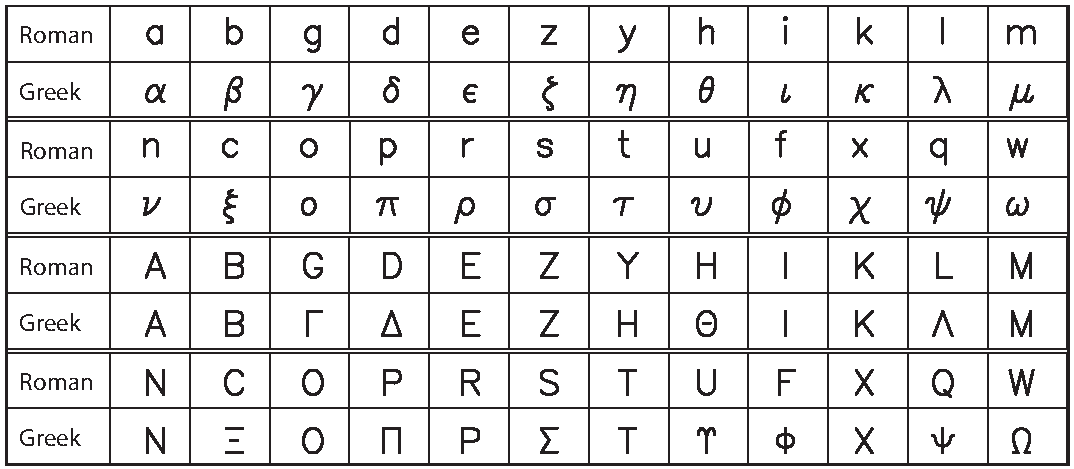
\includegraphics[width=5.0in]{greek.pdf}
  \caption[Roman to Greek Character Conversion]{Conversion for the string 
\vn{"{\B}g<r>"} where \vn{"<r>"} is a Roman character to the corresponding 
Greek character.}
\label{t:greek}
\end{table}

The parameters associated with data lines drawn in a graph are contained in the \vn{qp_line_struct}:
\begin{example}
  type qp_line_struct:
    width          = <integer>  ! Default = 1
    color          = <string>   ! Default = "black"
    pattern        = <string>   ! Default = "solid"
\end{example}

The possible colors for a line are given above. The \vn{pattern} parameter sets how the line is
drawn. Possible settings are:
\begin{example}
  solid      ! Solid line                 dotted     ! Dotted line             
  dashed     ! Dashed line                dash_dot3  ! Dash--dot--dot--dot line
  dash_dot   ! Dash--dot line
\end{example}
Pattern names are case insensitive.

The parameters associated with symbols that are drawn are contained in the \vn{qp_symbol_struct}:
\begin{example}
  type qp_symbol_struct:
    type          = <string>  ! Default = "dot"
    height        = <real>    ! Size in points. Default = 10
    color         = <string>  ! Default = "black"
    fill_pattern  = <string>  ! Default = "solid_fill"
    line_width    = <integer> ! Default = 1.
\end{example}

Possible \vn{fill_pattern} settings are:
\begin{example}
  solid_fill                    hatched           
  no_fill                       cross_hatched     
\end{example}
Fill pattern names are case insensitive.

The symbol types are:
\begin{example}
  square                 triangle                    square_concave              
  dot                    circle_plus                 diamond                     
  plus                   circle_dot                  star5                       
  times                  square_filled               triangle_filled           
  circle                 circle_filled               red_cross                 
  x                      star5_filled                star_of_david             
\end{example}
These symbols are illustrated in Table~\ref{t:plot.syms}. Symbol type names are case insensitive.

\begin{table}
  \centering
  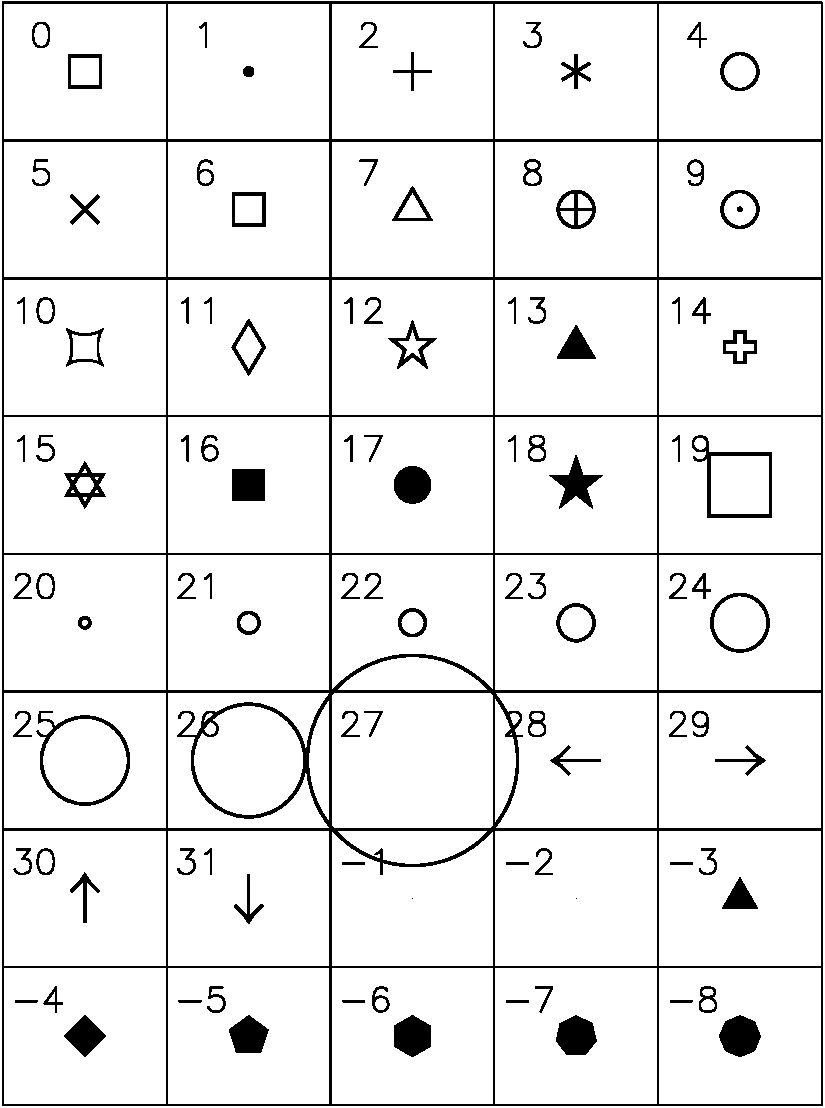
\includegraphics[width=5in]{plot-syms.pdf}
  \caption{Plotting Symbols.}
  \label{t:plot.syms}
\end{table}

\vfill
\break
